\documentclass[ignorenonframetext,xcolor=x11names]{beamer}

\input{../common.preamble.beamer.tex}
 
\title{Business 4720 - Class 12}

\subtitle{Supervised Machine Learning using R}

\begin{document}

\begin{frame}{}
  \titlepage
  \footnotesize
  \input{../license.tex}
\end{frame}

\section{Introduction}

\begin{frame}{This Class}

\begin{block}{What You Will Learn:}
\begin{itemize}
  \item Linear Regression Models in R
  \begin{itemize}
     \item Linear regression
     \item Lasso and Ridge regression
  \end{itemize}
  \item Classification Models in R
  \begin{itemize}
    \item Logistic Regression
    \item K-NN
  \end{itemize}
\end{itemize}
\end{block}
\end{frame}

\begin{frame}{Based On}
\small
\begin{block}{}
Gareth James, Daniel Witten, Trevor Hastie and Robert Tibshirani: \emph{An Introduction to Statistical Learning with Applications in R}. 2nd edition, corrected printing, June 2023. (ISLR2) \\
\vspace{1mm}
\url{https://www.statlearning.com} \\
\vspace{1mm}
Chapters 2, 3, 4, 5
\end{block}

\begin{block}{}
Trevor Hastie, Robert Tibshirani, and Jerome Friedman: \emph{The Elements of Statistical Learning}. 2nd edition, 12th corrected printing, 2017. (ESL) \\
\vspace{1mm}
\url{https://hastie.su.domains/ElemStatLearn/} \\
\vspace{1mm}
Chapters 2, 3, 4, 7
\end{block}

\begin{block}{}
Kevin P. Murphy: \emph{Probabilistic Machine Learning -- An Introduction}. MIT Press 2022. \\
\vspace{1mm}
\url{https://probml.github.io/pml-book/book1.html} \\
\vspace{1mm}
Chapters 4, 6, 9, 10, 11
\end{block}
\end{frame}

\begin{frame}{Linear Regression}

\begin{align*}
Y = \beta_0 + \beta_1 X + \epsilon
\end{align*}

\centering

\includegraphics[width=.8\textwidth]{../class11/Figures_Chapters_1-6/Chapter3/3_1.pdf} \\

\scriptsize Source: ISLR2 Figure 3.1
\end{frame}

\begin{frame}{Ensure a Linear Model is Sensible}
\centering
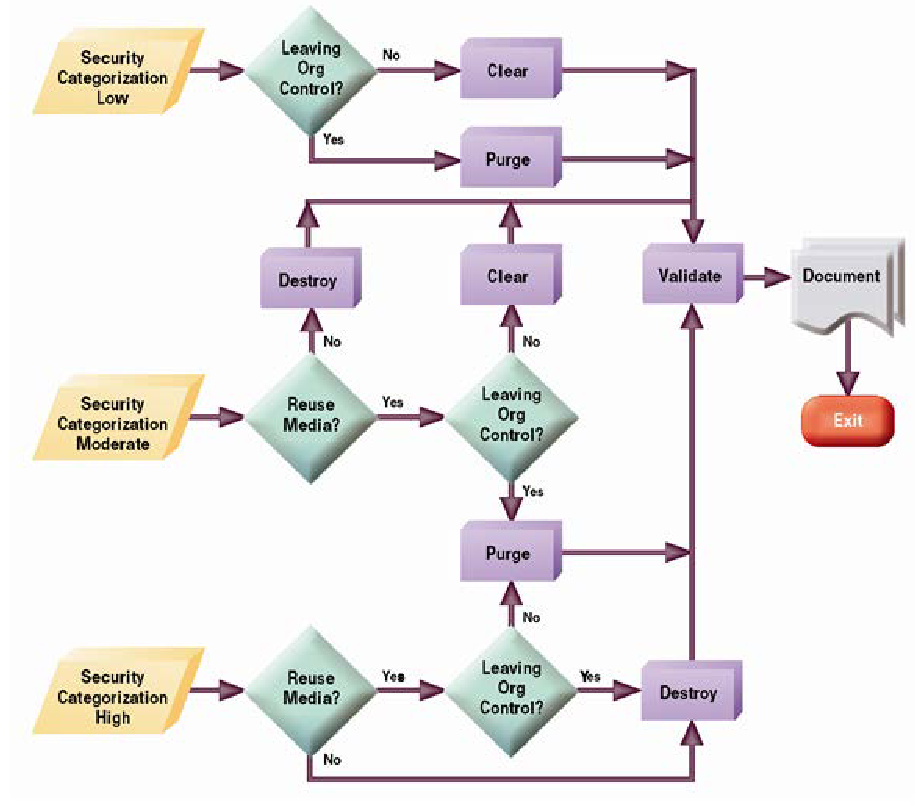
\includegraphics[width=.85\textwidth]{screen1.png} \\

\scriptsize Source: Murphy Figure 2.6 \\ \vspace{3mm}
\normalsize
The ''Datasaurus Dozen'': All datasets have the same correlation between the two variables!
\end{frame}

\begin{frame}{Correlation versus Regression}
\centering
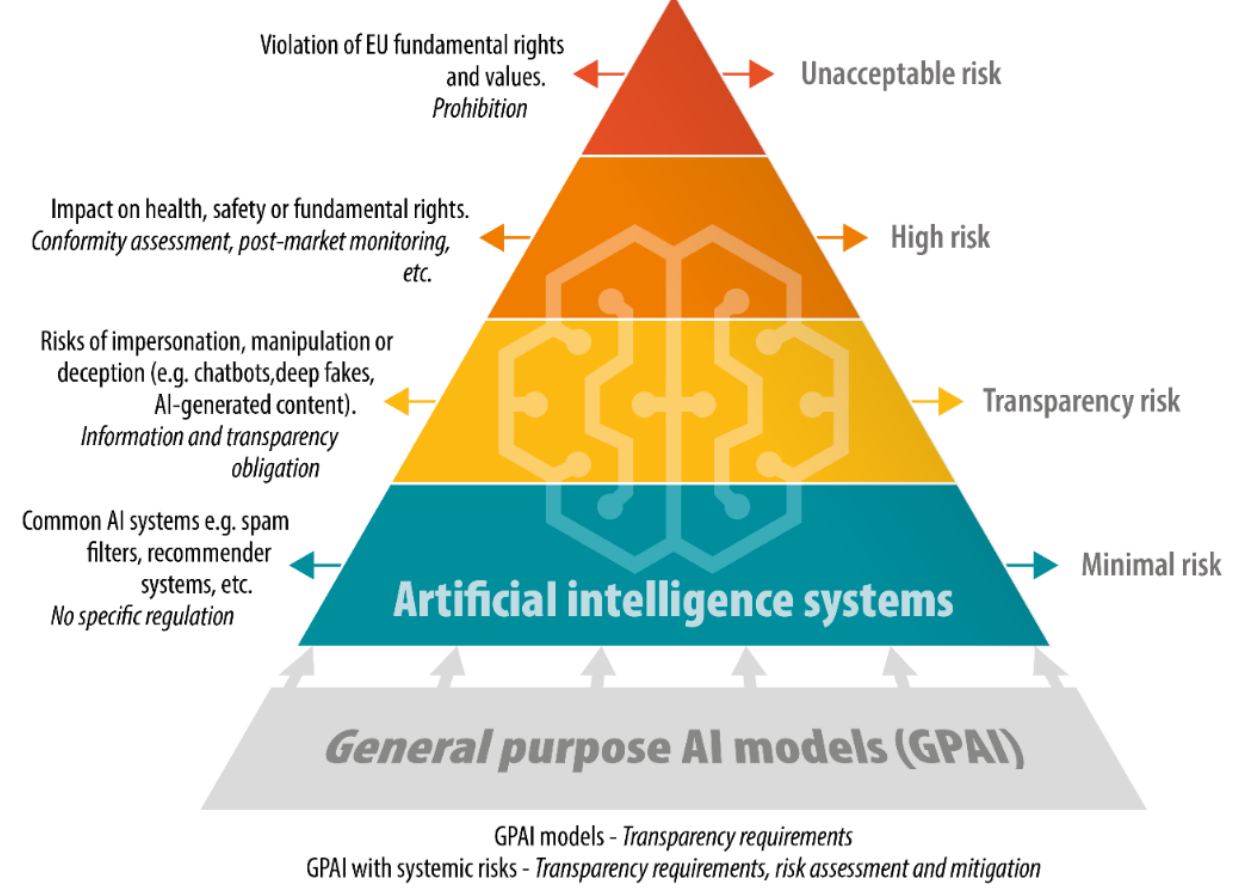
\includegraphics[width=.9\textwidth]{screen2.png} \\

\scriptsize Source: Murphy Figure 3.1 \\ \vspace{3mm}
\normalsize
Datasets with the same correlation (as indicated above each dataset) between two variables do not need to have the same regression slope!
\end{frame}


\begin{frame}{Estimating Linear Regression \small [cont'd]}
\begin{itemize}
  \item Estimate $\hat{\beta}_0$ and $\hat{\beta}_1$ to minimize the mean squared error (MSE) or residual sum of square (RSS)
\begin{align*}
\hat{y}_i &= \hat{\beta}_0 + \hat{\beta}_1 x_i \qquad \text{Predicted/fitted values} \\
RSS &= \sum_i \left( y_i - \hat{y}_i \right)^2  = \sum_i \left( y_i - \hat{\beta}_0 - \hat{\beta}_1 x_i \right)^2 \\
MSE &= \frac{1}{n} RSS
\end{align*}
  \item Analytically derivable \emph{least squares estimates} are
\begin{align*}
\hat{\beta}_1 &= \frac{\sum_i (x_i - \bar{x})(y_i - \bar{y})} {\sum_i (x_i - \bar{x})^2} \\
\hat{\beta}_0 &= \bar{y} - \hat{\beta}_1 \bar{x}
\end{align*}
where $\bar{x}$ and $\bar{y}$ are the sample means
%\item MSE (''L2 loss'') is susceptible to outlier influence, the MAE (''L1 loss'') is more robust
\end{itemize}
\end{frame}

\begin{frame}{Evaluating Linear Regression Models \small [cont'd]}
%\begin{itemize}
  %\item Estimates have \emph{standard errors} that indicate uncertainty of the estimates
  %\item A \emph{t-test} can be used to determine if a parameter is statistically significant from a value $V$ (typically $V=0$) using the test statistic
%\begin{align*}
%t = \frac{\hat{\beta}_1 - V}{SE(\hat{\beta}_1)}
%\end{align*}
  %\item The \emph{p-value} is the probability that the parameter is non-zero, assuming the estimated model is true
%  \item 
$R^2$ Value:
\begin{align*}
R^2 = \frac{TSS - RSS}{TSS} = 1 - \frac{RSS}{TSS}
\end{align*}
where $TSS = \sum_i(y_i - \bar{y})^2$ is the total sum of squares
\begin{block}{Interpretation}
\begin{enumerate}
  \item Proportion of explained variance
  \item Squared correlation of $Y$ and $\hat{Y}$
\end{enumerate}
\end{block}

%\end{itemize}
\end{frame}

\begin{frame}{Generalization to Multiple Predictors}
\begin{columns}
\begin{column}{0.65\textwidth}
\includegraphics[width=\textwidth]{../class11/Figures_Chapters_1-6/Chapter3/3_4.pdf}  \\
\scriptsize Source: ISLR2 Figure 3.4
\end{column}
\begin{column}{0.35\textwidth}
\begin{multline*}
Y = \beta_0 + \beta_1 X_1 + \beta_2 X_2 + \\
\cdots + \beta_p X_p + \epsilon
\end{multline*}
\end{column}
\end{columns}
\end{frame}

\begin{frame}{Regression with Qualitative Predictors}
\begin{itemize}
  \item Qualitative/categorical predictors (\emph{factors} with multiple, exclusive \emph{levels}) can be used in linear regression models using \textbf{dummy variables}:
\begin{align*}
x_{i1} = \begin{cases}
1 & \text{level ''a''} \\
0 & \text{else}
\end{cases} \\
x_{i2} = \begin{cases}
1 & \text{level ''b''} \\
0 & \text{else}
\end{cases} \\
x_{i3} = \begin{cases}
1 & \text{level ''c''} \\
0 & \text{else}
\end{cases}
\end{align*}
\item Note: $x_{i1} = x_{i2} = x_{i3} = 0$ represents level $d$!
%\item ''Contrasts'' determine how factor levels are coded using dummy variables
\end{itemize}
\end{frame}

\begin{frame}{Inputs, Predictors, and Polynomials}

Example:
\begin{align*}
Y = \beta_0 + \beta_1 X_1 + \beta_2 X_1^2 + \beta_3 X_2 + \beta_4 X_1 X_2 + \epsilon
\end{align*}
\begin{itemize}
  \item Still linear in $\beta_j$
  \item Two \textbf{inputs} $X_1$ and $X_2$
  \item Four \textbf{predictors} or \textbf{features}: $X_1$, $X_1^2$, $X_2$, $X_1 X_2$
  \item \textbf{Main effects} $\beta_1$ and $\beta_3$, 
  \item \textbf{Interaction effect} $\beta_4$, 
  \item A degree-2 \textbf{polynomial} effect $\beta_2$
\end{itemize}
\end{frame}

%\begin{frame}{Interactions}
%\centering

%\includegraphics[width=\textwidth]{../class11/Figures_Chapters_1-6/Chapter3/3_7.pdf}  \\

%\scriptsize Source: ISLR2 Figure 3.7
%\end{frame}

\begin{frame}{Multiple Regression with Polynomials}
\begin{columns}
\begin{column}{.7\textwidth}
\begin{center}
\includegraphics[width=\textwidth]{../class11/Figures_Chapters_1-6/Chapter3/3_8.pdf} \\

\scriptsize Source: ISLR2 Figure 3.8
\end{center}
\end{column}
\begin{column}{.3\textwidth}
\begin{itemize}
  \item Function more ''flexible''
  \item Fit to data improves
  \item Bias decreases
  \item Training MSE decreses (what about test MSE?)
\end{itemize}
\end{column}
\end{columns}
\end{frame}

\begin{frame}[fragile]{Linear Regression in R}
\small
Load libraries for data sets:
\begin{Rcode}
# Functions and data from the textbook # 'Modern 
# Applied Statistics with S'
library(MASS)
# Data sets from the textbook 'Introduction to 
# Statistical Learning with Applications in R'
library(ISLR2)
\end{Rcode}
The 'Boston' data set contains housing values in Boston in variable \texttt{medv} (median value). 

\begin{Rcode}
Examine the data:

# Get a description of the data
?Boston

# Get a summary and first few rows
summary(Boston)
head(Boston)

# Bivariate scatterplots
plot(Boston)
\end{Rcode}
\end{frame}

\begin{frame}[fragile]{Linear Regression in R \small [cont'd]}
\small
Fit a simple model, examine and plot the results:
\begin{Rcode}
# Fit a model with intercept only
fitted.model <- lm(medv ~ 1, data=Boston)
summary(fitted.model)

# Fit a model with predictor lstat
fitted.model <- lm(medv ~ lstat, data=Boston)
summary(fitted.model)

# Plot the data and the regression line
plot(medv ~ lstat, data=Boston)
abline(fitted.model, lwd=3, col='red')
\end{Rcode}
\end{frame}

\begin{frame}[fragile]{Linear Regression in R \small [cont'd]}
\small
The \texttt{predict()} function calculates $\hat{y}_i$:

\begin{Rcode}
# For training data
y.hat <- predict(fitted.model, Boston)

# For new data
newData <- data.frame(lstat = c(5, 10, 15))
predict(fitted.model, newData)
\end{Rcode}

The \texttt{residuals()} function calculates $y_i - \hat{y}_i$:
\begin{Rcode}
# Plot the residuals against predicted values
plot(predict(fitted.model), residuals(fitted.model))
\end{Rcode}
\end{frame}

\begin{frame}[fragile]{Linear Regression in R \small [cont'd]}
\small
Build more complex models:
\begin{Rcode}
# Add another predictor
fitted.model <- lm(medv ~ lstat + age, data=Boston)

# Add all main effects
fitted.model <- lm(medv ~ ., data=Boston)

# Add interaction terms
fitted.model <- lm(medv ~ lstat + age + lstat:age,data=Boston)
   
# Shorter and equivalent
fitted.model <- lm(medv ~ lstat*age, data=Boston)
summary(fitted.model)
\end{Rcode}
\end{frame}

\begin{frame}[fragile]{Linear Regression in R \small [cont'd]}
\small
Add polynomial terms:
\begin{Rcode}
# Add a polynomial term; use the I(.) function
# for any data transformations, such as log(),
# or exp() or sqrt() as well as polynomials
fitted.model <- lm(medv ~ lstat + I(lstat^2), data=Boston)
summary(fitted.model)

# Add all polynomial terms up to degree 5
fitted.model <- lm(medv ~ poly(lstat, 5), data=Boston)

# Note the coefficients for the polynomials in the summary
summary(fitted.model)
\end{Rcode}
\end{frame}

%\begin{frame}[fragile]{Linear Regression in R \small [cont'd]}
%Categorical predictors (''factors'') using dummy variables:
%\begin{Rcode}
%?Carseats
%\end{Rcode}
%Identify factor/categorical variables and their levels:
%\begin{Rcode}
%is.factor(Carseats$ShelveLoc)
%levels(Carseats$ShelveLoc)
%levels(Carseats$Urban)
%levels(Carseats$US)
%\end{Rcode}
%\textbf{Contrasts} show the dummy variables created (columns) and the values they take for different  factor levels (row):
%\begin{Rcode}
%contrasts(Carseats$ShelveLoc)
%contrasts(Carseats$US)
%\end{Rcode}
%Fit the model:
%\begin{Rcode}
%summary(lm(Sales ~ . , data=Carseats))
%\end{Rcode}
%\end{frame}


\begin{frame}{Hands-On Exercises}
{\small (Source: ISLR2 Chapter 3)}
\small
Use the \texttt{Auto} data set from the ISLR2 library with \texttt{mpg} as the target.
  \begin{enumerate}
     \item Perform a linear regression with \texttt{horsepower} as predictor
     \item Is there a relationship between the predictor and target? What form and how strong?
     \item What is the predicted \texttt{mpg} value for a \texttt{horsepower} of 98? 
     \item Plot the response and predictor. Use the \texttt{abline()} function to add the regression line
     \item Produce a scatterplot of all variables
     \item Perform a linear regression of all main effects (except for the variable \texttt{name})
     \item Use the \texttt{*} and \texttt{:} symbols to add interaction effects.
     \item Add transformations of the predictors (using the \texttt{I(.)} function) such as $\log(X)$, $\sqrt{X}$, $X^2$.
  \end{enumerate}
\end{frame}

%\begin{frame}{Hands-On Exercises}
%{\small (Source: ISLR2 Chapter 3)}
%\small
%Use the \texttt{Carseats} data set from the ISLR2 library with \texttt{Sales} as the target.
  %\begin{enumerate}
     %\item Perform a linear regression with \texttt{Price}, \texttt{Urban} and \texttt{US} as predictors
     %\item Interpret the coefficients. Tip: Some variables are categorical
     %\item Remove non-significant predictors
     %\item How well do the two models fit the data?
  %\end{enumerate}
%\end{frame}

\begin{frame}[fragile]{Cross-Validation in R -- Holdout Sample}
Validation set approach:
\begin{Rcode}
# Randomly use half the Auto data as training sample
train.idx <- sample(nrow(Auto), nrow(Auto)/2)
train.data <- Auto[train.idx,]
test.data <- Auto[-train.idx,]

# Fit model to (train model on) a subset
fitted.model <- lm(mpg ~ horsepower, data=train.data)

# Calculate the training data MSE
mean((train.data$mpg - predict(fitted.model, train.data))^2)

# Calculate the validation data MSE
mean((test.data$mpg - predict(fitted.model, test.data))^2)
\end{Rcode}
\end{frame}

\begin{frame}[fragile]{Cross-Validation in R}
K-Fold Cross-Validation with $K=5$:
\begin{Rcode}
library(boot)

# Fit a model with glm and show its summary
glm.fit <- glm(mpg ~ horsepower, data=Auto)

# 5-fold CV
cv.err <- cv.glm(Auto, glm.fit, K=5)
cv.err$delta[1]
\end{Rcode}
LOOCV is K-Fold CV with $K=N$

\begin{Rcode}
# LOOCV is k-fold CV where K equals N, num of obs
cv.err <- cv.glm(Auto, glm.fit, K=nrow(Auto))
cv.err$delta[1]
\end{Rcode}
%\begin{itemize}
%\scriptsize
  %\item The \texttt{glm()} function fits \emph{Generalized Linear Models} using maximum-likelihood estimation, not RSS minimization. They yield identical solutions for ''ordinary'' linear models but MLE is more flexible and can be used on a wide range of models. The use of \texttt{glm()} is identical to that of \texttt{lm()} for ''ordinary'' linear models; the \texttt{boot} package provides cross-validation for \texttt{glm} models
%\end{itemize}
\end{frame}


%\begin{frame}[fragile]{Cross-Validation in R -- K-Fold CV}

%\textbf{Example:} Use cross-validation to compare different models:

%\begin{Rcode}
%set.seed(17)
%cv.err <- rep(0, 5)
%for(i in 1:20) {
  %glm.fit <- glm(mpg ~ poly(horsepower,i), data=Auto)
  %cv.err[i] <- cv.glm(Auto, glm.fit, K=10)$delta[1]
%}
%cv.err
%\end{Rcode}
%\end{frame}


\begin{frame}{Hands-On Exercises -- Cross-Validation}
Consider the Boston housing data set \texttt{Boston}.
\begin{enumerate}
  \item Fit a regression model using \texttt{medv} as target, and \texttt{age}, \texttt{lstat}, and \texttt{ptratio} as predictors
  \item Using the validation set approach, compute the test error of this model. Perform the following steps
  \begin{enumerate}
     \item Split the data set using 75\% for training and 25\% for testing
     \item Fit the model to training data
     \item Predict the target for the testing data
     \item Compute the test error
  \end{enumerate}
  \item Repeat the previous step 2 times, using different splits. How do the results change?
  \item Average the test error of the four splits. 
  \item Calculate the test error estimate using LOOCV. Compare your result to that of step 4.
  \item Calculate the test error estimate using 10-fold cross-validation. Compare the estimate to that of step 4
\end{enumerate}
\end{frame}

\begin{frame}{Shrinkage Methods}
\begin{block}{Goals}
\begin{itemize}
   \item Avoid overfitting
   \item Reduce variance
   \item ''Shrink'' regression coefficients towards zero
   \item Penalize coefficients that are ''too high''
   \item Type of ''\textbf{regularization}'' (methods to prevent overfitting)
\end{itemize}
\end{block}
\end{frame}


\begin{frame}{Ridge Regression}{a.k.a Tikhonov Regularization}
\begin{align*}
\text{Minimize} \quad RSS + \lambda \sum_{j=1}^p \beta_j^2 = RSS + \lambda ||\beta||_2^2
\end{align*}
\begin{itemize}
   \item L2 regularizer (it penalizes the L2 norm of $\beta$)
   \item Parameter $\lambda$ controls the amount of shrinkage
   \item Larger $\lambda$ reduce variance but increase bias
   \item Not scale invariant: Standardize predictors
\end{itemize}
\end{frame}

\begin{frame}{Ridge Regression}{a.k.a Tikhonov Regularization}
\includegraphics[width=\textwidth]{../class11/Figures_Chapters_1-6/Chapter6/6_5.pdf}

\scriptsize Source: ISLR2 Figure 6.5 \normalsize \\

\begin{itemize}
  \item Bias
  \item \color{teal}Variance
  \item \color{magenta}MSE
\end{itemize}

\end{frame}

\begin{frame}{Ridge Regression Example }{Fitting a Degree 14 Polynomial}
\centering
\includegraphics[width=0.9\textwidth]{screen4.png}\\
\scriptsize Source: Murphy Figure 4.5
\end{frame}

\begin{frame}{Lasso regression}{''Least Absolute Shrinkage and Selection Operator''}
\begin{align*}
\text{Minimize} \quad RSS + \lambda \sum_{j=1}^p |\beta_j| = RSS + \lambda ||\beta||_1
\end{align*}
\begin{itemize}
   \item L1 regularizer (it penalizes the L1 norm of $\beta$)
   \item Lasso may exclude variables by forcing their $\beta_j$ to 0
   \item Parsimonious, more interpretable models than ridge regression
\end{itemize}
\begin{columns}
\begin{column}{0.8\textwidth}
\includegraphics[width=\textwidth]{../class11/Figures_Chapters_1-6/Chapter6/6_6.pdf}
\end{column}
\begin{column}{0.2\textwidth}
\scriptsize Source: ISLR2 Figure 6.6
\end{column}
\end{columns}
\end{frame}


\begin{frame}{Elastic Net}
The Elastic Net penalty is a mix of L1-norm $||\beta||_1$ and L2-norm $||\beta||_2^2$ penalties, defined by $\alpha$:
\begin{align*}
\lambda \left( \alpha ||\beta||_1  + (1-\alpha)||\beta||_2^2 \right)
\end{align*}
\vspace{-.5\baselineskip}
\begin{itemize}
\item $\alpha = 0$: Ridge regression
\item $\alpha = 1$: Lasso
\end{itemize}

\vspace{.5\baselineskip}
The \texttt{glmnet()} function in the \texttt{glmnet} library for R uses the Elastic Net regularization method.\end{frame}

\begin{frame}[fragile]{Ridge Regression in R}
\small

Use the \texttt{Hitters} data set to model \texttt{Salary} as outcome and other variables as predictors.
\begin{Rcode}
library(ISLR2)
library(glmnet)

# Remove missing values
Hitters <- na.omit(ISLR2::Hitters)
\end{Rcode}

The \texttt{glmnet()} function requires separate $x$ and $y$ values, instead of a formula. To create dummy variables for categorical variables, use the \texttt{model.matrix()} function:

\begin{Rcode}
# Create dummy variables for categorical variables
# Remove intercept from model
x <- model.matrix(Salary ~ ., Hitters)[, -1]
y <- Hitters$Salary
\end{Rcode}
\end{frame}

\begin{frame}[fragile]{Ridge Regression in R \small [cont'd]}
Example for $\lambda=10$ using \texttt{glmnet()} with $\alpha=0$:
\begin{Rcode}
ridge.model <- glmnet(x, y, alpha=0, lambda=10)
\end{Rcode}
Examine coefficients:
\begin{Rcode}
coef(ridge.model)
\end{Rcode}
Examine L2 norm (penalty to RSS) (without intercept):
\begin{Rcode}
L2.norm = sqrt(sum(coef(ridge.model)[-1]^2))
\end{Rcode}
Examine MSE:
\begin{Rcode}
mean((y-predict(ridge.model, x))^2)
\end{Rcode}
\end{frame}

%\begin{frame}[fragile]{Ridge Regression in R \small [cont'd]}
%\small
%Set up a sequence of $\lambda$ to try and fit the model for each $\lambda$:
%\begin{Rcode}
%# Set up the sequence of lambda values to try
%grid <- 10^seq(from=10, to=-2, length=100)
%print(grid)
%ridge.model <- glmnet(x, y, alpha=0, lambda=grid)
%\end{Rcode}
%Examine some results:
%\begin{Rcode}
%# Select the 50th lambda value
%ridge.model$lambda[50]
%coef(ridge.model)[, 50]
%L2.norm = sqrt(sum(coef(ridge.model)[-1, 50]^2))

%# Select the 60th lambda value
%ridge.model$lambda[60]
%coef(ridge.model)[, 60]
%L2.norm = sqrt(sum(coef(ridge.model)[-1, 60]^2))
%\end{Rcode}
%\end{frame}

\begin{frame}{Selecting the Tuning Parameter}
\begin{block}{Grid Search}
\begin{itemize} 
   \item Define a set/range of possible values for $\lambda$
   \item Cross-validate models for each value of $\lambda$
   \item Fit the final model to the optimal cross-validated error
\end{itemize}
\end{block}

\vspace{\baselineskip}
\centering
\includegraphics[width=\textwidth]{../class11/Figures_Chapters_1-6/Chapter6/6_13.pdf} \\

\scriptsize Source: ISLR2 Figure 6.13
\end{frame}

\begin{frame}[fragile]{Ridge Regression in R -- Optimal Lambda}
\small
Create holdout test data set:
\begin{Rcode}
# Randomly split the Hitters data
train.idx <- sample(nrow(Hitters), nrow(Hitters)/2)
x.train <- x[train.idx,]
x.test <- x[-train.idx,]
y.train <- y[train.idx]
y.test <- y[-train.idx]
\end{Rcode}
Use the training set to find optimal $\lambda$ with CV:
\begin{Rcode}
# 5-fold cross-validation, use MSE as metric
cv.out <- cv.glmnet(x.train, y.train, alpha=0, 
                    nfolds=5, type.measure='mse')
\end{Rcode}
\end{frame}


\begin{frame}[fragile]{Ridge Regression in R  -- Optimal Lambda \small [cont'd]}
\small
Show the optimal lambda, the MSE and its standard error, and the number of non-zero coefficients.
\begin{columns}
\begin{column}{.35\textwidth}
\begin{Rcode}
print(cv.out)
plot(cv.out)
lambda.opt <- 
  cv.out$lambda.min
\end{Rcode}
\end{column}
\begin{column}{.65\textwidth}
\begin{textcode}
> print(cv.out)
    Lambda Index Measure    SE Nonzero
min  461.6    68  102536 13016      19
1se 2244.8    51  114493 19007      19
\end{textcode}
\end{column}
\end{columns}
\includegraphics[width=\textwidth]{crossvalidated_ridge.pdf}
\end{frame}

\begin{frame}[fragile]{Ridge Regression in R -- Optimal Lambda \small [cont'd]}
\small
Fit test data using optimal $\lambda$:
\begin{Rcode}
ridge.model <- glmnet(x.test, y.test, 
                      alpha=0, lambda=lambda.opt)
\end{Rcode}
Compare coefficients between ridge and unpenalized least squares:
\begin{Rcode}
coef(ridge.model)
coef(lm(y.test ~ x.test + 1))
\end{Rcode}
\end{frame}

\begin{frame}[fragile]{Ridge Regression in R -- Prediction}
\small
Predict values for the test data set:
\begin{Rcode}
y.hat.test <- predict(ridge.model, newx=x.test, 
                                      type='response')
\end{Rcode}
Calculate test MSE to compare to the CV optimal MSE above:
\begin{Rcode}
mean((y.hat.test - y.test)^2)
\end{Rcode}
Recall, the CV cross-validated error on the training set is an estimate/approximation of the real test error.
\end{frame}

\begin{frame}[fragile]{The Lasso in R \small [cont'd]}
\small
Example for $\lambda=10$ using \texttt{glmnet()} with $\alpha=1$:
\begin{Rcode}
lasso.model <- glmnet(x, y, alpha=1, lambda=10)
\end{Rcode}
Examine coefficients:
\begin{Rcode}
coef(lasso.model)
\end{Rcode}
Examine L1 norm (penalty to RSS) (without intercept):
\begin{Rcode}
L1.norm = sum(abs(coef(lasso.model)[-1])))
\end{Rcode}
Examine MSE:
\begin{Rcode}
mean((y-predict(ridge.model, x))^2)
\end{Rcode}

Use the training set to find optimal $\lambda$ with CV:
\begin{Rcode}
# 5-fold cross-validation, use MSE as metric
cv.out <- cv.glmnet(x.train, y.train, alpha=1, 
                    nfolds=5, type.measure='mse')
\end{Rcode}
\end{frame}

\begin{frame}[fragile]{The Lasso in R -- Optimal Lambda}
\small
Show the optimal lambda, the MSE and its standard error, and the number of non-zero coefficients.
\begin{columns}
\begin{column}{.35\textwidth}
\begin{Rcode}
print(cv.out)
plot(cv.out)
lambda.opt <- 
  cv.out$lambda.min
\end{Rcode}
\end{column}
\begin{column}{.65\textwidth}
\begin{textcode}
> print(cv.out)
    Lambda Index Measure    SE Nonzero
min  33.33    22  107161 17195       6
1se  92.75    11  122071 22061       4
\end{textcode}
\end{column}
\end{columns}
Note the number of non-zero coefficients in the result:
\begin{center}
\includegraphics[width=.8\textwidth]{crossvalidated_lasso.pdf}
\end{center}
\end{frame}

\begin{frame}[fragile]{The Lasso in R -- Prediction}
Fit test data using optimal $\lambda$:
\begin{Rcode}
lasso.model <- glmnet(x.test, y.test, 
                         alpha=1, lambda=lambda.opt)
\end{Rcode}
Compare coefficients between Lasso and unpenalized least squares:
\begin{Rcode}
coef(lasso.model)
coef(lm(y.test ~ x.test + 1))
\end{Rcode}
Predict values for the test data set and compute test MSE
\begin{Rcode}
y.hat.test <- predict(lasso.model, newx=x.test, 
                                      type='response')
mean((y.hat.test - y.test)^2)
\end{Rcode}
\end{frame}

\begin{frame}{Hands-On Exercises -- Shrinkage Methods}{Source: ISLR2, Chapter 6}
Predict the number of applications received using the other variables in the \texttt{College} dataset
  \begin{enumerate} 
      \item Split the data set into a training and a test set
      \item Fit an unpenalized linear model on the training set. Report the test error.
      \item Fit a ridge regression model on the training set, with $\lambda$ chosen by cross-validation. Report the test error.
      \item Fit a lasso model on the training set, with $\lambda$ chosen by cross-validation. Report the test error.
      \item Compare and contrast the results
  \end{enumerate}
\end{frame}

\begin{frame}{Hands-On Exercises -- Shrinkage Methods}{Source: ISLR2, Chapter 6}
Predict the per-capita crime rate in the \texttt{Boston} data set using the other variables.
  \begin{enumerate}
      \item Split the data set into a training and a test set
      \item Fit an unpenalized linear model on the training set. Report the test error.
      \item Fit a ridge regression model on the training set, with $\lambda$ chosen by cross-validation. Report the test error.
      \item Fit a lasso model on the training set, with $\lambda$ chosen by cross-validation. Report the test error.
      \item Compare and conrast the results
  \end{enumerate}
\end{frame}

%\begin{frame}{Robust Regression}
%\begin{block}{Problem}
%\begin{itemize}
   %\item MSE loss function susceptible to outliers (quadratic error)
%\end{itemize}
%\end{block}
%\begin{block}{Huber loss}
%\begin{align*}
   %L_{\text{huber}}(r, \delta) = \begin{cases}
   %r^2/2 \quad &\text{if} |r| \leq \delta \\
   %\delta |r| - \delta^2/2 \quad &\text{if} |r| > \delta
%\end{cases}
%\end{align*}
%\begin{itemize}
   %\item L2 error (MSE) for small errors $\leq \delta$
   %\item L1 error (MAE) for large errors $> \delta$
   %\item Identify optimal $\delta$ through cross-validation
%\end{itemize}
%\end{block}
%\end{frame}

\begin{frame}{Classification}
  \begin{itemize}
     \item Qualitative (categorical) outcome
     \item Estimate or predict probabilities of class membership
     \item \textbf{Problem}: Linear combinations of predictors not in $[0, 1]$
     \item \textbf{Solution}: ''Link'' function transforms linear combinations of predictors
  \end{itemize}
\includegraphics[width=\textwidth]{../class11/Figures_Chapters_1-6/Chapter4/4_2.pdf}
\scriptsize Source: ISLR2 Figure 4.2
\end{frame}

\begin{frame}{Logistic Regression}
\begin{block}{Logistic / Sigmoid Function}
\begin{columns}
\begin{column}{0.6\textwidth}
\begin{align*}
  \sigma(a) &= \frac{1}{1 + e^{-a}} = \frac{e^a}{1 + e^a} %\\
%  &= 1 - \sigma(-a)
\end{align*}
\end{column}
\begin{column}{0.4\textwidth}
\includegraphics[height=.8in]{logistic.png}
\end{column}
\end{columns}
\end{block}

\begin{block}{Binary Case (Binomial Logistic Regression)}
\small
\begin{align*}
p(X) = \sigma( \beta_0 + \beta_1 X) &= \frac{e^{\beta_0 + \beta_1 X}}{1 + e^{\beta_0 + \beta_1 X}} %\\
%\Rightarrow \quad \frac{p(X)}{1 - p(X)} &= e^{\beta_0 + \beta_1 X} \qquad\;\; \text{\textbf{''Odds''}} \\
%\Rightarrow \quad \log \left( \frac{p(X)}{1 - p(X)} \right) &= \beta_0 + \beta_1 X \qquad \text{\textbf{''Log-Odds'', ''Logits''}}
\end{align*}
where the linear predictor $\beta_0 + \beta_1 X$ are the \textbf{logits}
\end{block}
\end{frame}

\begin{frame}{Logistic Regression \small [cont'd]}
\begin{block}{Predictions}
Given estimates $\hat{\beta}_0$ and $\hat{\beta}_1$, use the link function to predict class/outcome probabilities for observation $X$:
\begin{align*}
  \hat{p}(X) = \frac{e^{\hat{\beta}_0 + \hat{\beta}_1 X}}{1 + e^{\hat{\beta}_0 + \hat{\beta}_1 X}}
\end{align*}
\end{block}
\begin{block}{Multinomial Logistic Regression}
\begin{itemize}
  \item Same mathematical form
  \item Probability for class being $k$:
\begin{align*}
\Rightarrow \Pr(Y=k|X) &= \frac{e^{\beta_{k0}+\beta_{k1}x_1 + \cdots + \beta_{kp}x_p}}{1 + \sum_{l=1}^{K-1} e^{\beta_{l0}+\beta_{l1}x_1 + \cdots + \beta_{lp}x_p}}
\end{align*}
\end{itemize}
\end{block}
\end{frame}

%\begin{frame}{Logistic Regression \small [cont'd]}
%\begin{itemize}
   %\item Multiple $p$ predictors: \textbf{Multiple Linear Regression}
   %\item Multiple $K$ classes: \textbf{Multinomial Logistic Regression}
   %\item Multiple $n$ labels: \textbf{Multi-label Classification}
%\end{itemize}
%\end{frame}

%\begin{frame}{Multinomial Logistic Regression}
%\small
%\begin{align*}
%\log \left( \frac{\Pr(Y=k | X=x)}{\Pr(Y=K | X=x)}\right) &= \beta_{k0}+\beta_{k1}x_1 + \cdots + \beta_{kp}x_p \; , k<K \\
%\intertext{Exponentiating and rearranging:}
%\Pr(Y=k | X=x) &= \Pr(Y=K | X=x) e^{\beta_{k0}+\beta_{k1}x_1 + \cdots + \beta_{kp}x_p} \;, k<K\\
%\intertext{Because probabilities must sum to 1:}
%\Pr(Y=K | X=x) &= 1 - \sum_{l=1}^{K-1} \Pr(Y=l | X=x) \\
%&= 1 - \sum_{l=1}^{K-1} \Pr(Y=K | X=x) e^{\beta_{k0}+\beta_{k1}x_1 + \cdots + \beta_{kp}x_p} \\
%\Rightarrow \Pr(Y=K | X = x) &= \frac{1}{1 + \sum_{l=1}^{K-1} e^{\beta_{k0}+\beta_{k1}x_1 + \cdots + \beta_{kp}x_p}} \\
%\Rightarrow \Pr(Y=k|X=x) &= \frac{e^{\beta_{k0}+\beta_{k1}x_1 + \cdots + \beta_{kp}x_p}}{1 + \sum_{l=1}^{K-1} e^{\beta_{l0}+\beta_{l1}x_1 + \cdots + \beta_{lp}x_p}} \;, \; k < K
%\end{align*}
%\end{frame}

\begin{frame}{Logistic Regression with Polynomials}
Transforming decision boundaries:
\begin{center}
\includegraphics[width=\textwidth]{Figure_10.3.png} \\
\scriptsize Source: Murphy Figure 10.3
\end{center}
\end{frame}

\begin{frame}{Logistic Regression with Polynomials \small [cont'd]}
But beware of overfitting:
\begin{center}
\includegraphics[width=.8\textwidth]{screen3.png} \\
\scriptsize Source: Murphy Figure 10.4
\end{center}
\end{frame}

\begin{frame}[fragile]{Logistic Regression in R}
\small
Use the stock market data set \texttt{Smarket} to predict the binary outcome \texttt{Direction} (the direction of market changes, up or down) using prior returns as predictors:
\begin{Rcode}
library(ISLR2)
?Smarket
\end{Rcode}
%Contrasts show how factor levels are encoded using dummy variables:
%\begin{Rcode}
%contrasts(Smarket$Direction)
%\end{Rcode}
Fit to full data set. Note the link function in the \texttt{family} argument for the \texttt{glm()} function:
\begin{Rcode}
logreg.fitted <- 
   glm(Direction ~ Lag1 + Lag2 + Lag3 + Lag4 + Lag5 + Volume, 
       data=Smarket, 
       family=binomial(link='logit'))
summary(logreg.fitted)
\end{Rcode}
\end{frame}


\begin{frame}[fragile]{Logistic Regression in R}
\small
Use \texttt{predict()} to predict logits for data set:
\begin{Rcode}
logreg.logits <- predict(logreg.fitted, newdata = Smarket)
\end{Rcode}
Use \texttt{predict()} to predict probabilities for data set:
\begin{Rcode}
# Predict probabilities for training test
logreg.probs <- predict(logreg.fitted, newdata = Smarket, 
                     type='response')
\end{Rcode}
Make classificiation decision using decision rule:
\begin{Rcode}
# Predict 'up' or 'down' based on probabilities
# and a fixed threshold
pred.direction <- rep(NA, nrow(Smarket))
pred.direction[logreg.probs >  .5] <- 'Up'
pred.direction[logreg.probs <= .5] <- 'Down'
\end{Rcode}
\end{frame}

\begin{frame}[fragile]{Logistic Regression in R}
\small
Compute confusion matrix:
\begin{Rcode}
# Compute confusion matrix
logreg.cm <- table(pred.direction, Smarket$Direction)
print(logreg.cm)
\end{Rcode}
Compute accuracy as mean of correct classifications:
\begin{Rcode}
# Compute accuracy
mean(pred.direction == Smarket$Direction)
\end{Rcode}
\end{frame}

\begin{frame}[fragile]{Logistic Regression in R -- Holdout Set} 
\small
Split data to train and test set. Because this is time-dependent data, split by time to avoid mixing past and future data:
\begin{Rcode}
train.data <- Smarket[Smarket$Year < 2005,]
test.data <- Smarket[!(Smarket$Year < 2005),]
\end{Rcode}
Fit model to training set:
\begin{Rcode}
logreg.fitted <- 
   glm(Direction~Lag1+Lag2+Lag3+Lag4+Lag5+Volume, 
       data=train.data, family=binomial(link='logit'))
\end{Rcode}
Predict probabilities for test data:
\begin{Rcode}
logreg.probs <- predict(logreg.fitted, 
    newdata = test.data, type='response')
\end{Rcode}
Make classification decision using decision rule:
\begin{Rcode}    
pred.direction <- rep(NA, nrow(test.data))
pred.direction[logreg.probs >  .5] <- 'Up'
pred.direction[logreg.probs <= .5] <- 'Down'
\end{Rcode}
\end{frame}

\begin{frame}[fragile]{Logistic Regression in R -- Holdout Set} 
\small
Compute confusion matrix for test data:
\begin{Rcode}
logreg.cm <- table(pred.direction, test.data$Direction)
print(logreg.cm)
\end{Rcode}
Calculate accuracy as the mean of correct classifications:
\begin{Rcode}
mean(pred.direction == test.data$Direction)
\end{Rcode}
\end{frame}

\begin{frame}[fragile]{Logistic Regression in R -- Evaluation}
\small
Using the \texttt{ROCR} library for classifier evaluation:
\begin{Rcode}
library(ROCR)

# A prediction object collects predicted 
# probabilities and true labels
pred.obj <- prediction(logreg.probs, 
                       test.data$Direction)

# Get some classifier performance metrics
# ROCR varies the threshold.
plot(performance(pred.obj, 'acc'))
plot(performance(pred.obj, 'prec'))
plot(performance(pred.obj, 'rec'))
plot(performance(pred.obj, 'f'))
performance(pred.obj, 'auc')@y.values[[1]]
\end{Rcode}
\end{frame}

\begin{frame}[fragile]{Logistic Regression in R -- Evaluation}
\small
continued \ldots
\begin{Rcode}
# ROC - True positive rate versus false positive rate
plot(performance(pred.obj, 'tpr', 'fpr'), colorize=T)
abline(0, 1)

# Precision/Recall plot
plot(performance(pred.obj, 'prec', 'rec'), colorize=T)
\end{Rcode}

\begin{columns}
\begin{column}{.4\textwidth}
\includegraphics[width=\textwidth]{roc.pdf}
\end{column}
\begin{column}{.4\textwidth}
\includegraphics[width=\textwidth]{precrec.pdf}
\end{column}
\end{columns}
\end{frame}


\begin{frame}{Naive Bayes Classifier}
\small \vspace{-3mm}
\begin{itemize}
\item \textbf{Bayes Theorem}:
\begin{align*}
\Pr(Y=c\, | X) &= \frac{p(X|Y=c)\, p(Y=c)}{p(X)} \\
&= \frac{p(X|Y=c)\,p(Y=c) }{\sum_{l=1}^K p(X|Y=l)\,p(Y=l)} 
\end{align*}
\item \textbf{Naive Bayes Assumption}: Within each class $c$, the $D$ predictors are independent:
\begin{align*}
p(X | Y=c ) &= p(x_1 | Y=c) \times p(x_2 | Y=c) \times \cdots  \times p(x_D | Y=c) \\
            &= \prod_{d=1}^D p(x_d | Y=c)
\end{align*}
\item \textbf{Posterior probability}:
\begin{align*}
p(Y=c|X) &= \frac{\left(\prod_{d=1}^D p(x_d | Y=c)\right) \, p(Y=c)}{\left(\sum_{l=1}^K \prod_{d=1}^D p(x_d | Y=l)\right) \, p(Y=l) } 
\end{align*}
\end{itemize}
\end{frame}


\begin{frame}[fragile]{Naive Bayes Classifier in R}
\small
Naive Bayes using the \texttt{naiveBayes} function in the \texttt{e1071} library:
\begin{Rcode}
library(e1071)

# Fit using same syntax as glm
nb.fitted <- naiveBayes(Direction~Lag1+Lag2, data=train.data)

# Output contains prior and conditional probabilities (and SD)
nb.fitted
\end{Rcode}
Predict class membership and compute confusion matrix:
\begin{Rcode}
nb.predictions <- predict(nb.fitted, test.data)
nb.cm <- table(nb.predictions, test.data$Direction)
print(nb.cm)
\end{Rcode}
\end{frame}

\begin{frame}[fragile]{Naive Bayes Classifier in R -- Evaluation}
\small
Evaluate the classifier:
\begin{Rcode}
# Predict probabilities (for use with ROCR)
nb.probs <- predict(nb.fitted, test.data, type='raw')

# Create an ROCR prediction object
nb.pred.obj <- prediction(nb.probs[,'Up'], 
                          test.data$Direction)
\end{Rcode}
Assess ROC and AUC:
\begin{Rcode}
# Generate an ROC plot
plot(performance(nb.pred.obj, 'tpr', 'fpr'), colorize=T)
abline(0, 1)

# Compute the AUC
performance(nb.pred.obj, 'auc')@y.values[[1]]
\end{Rcode}
\end{frame}

\begin{frame}{Naive Bayes Classifier in R -- Evaluation}
\centering
\includegraphics[height=2.5in]{nb_roc.pdf}
\end{frame}

\begin{frame}[fragile]{KNN Classification in R}
\small
Using the \texttt{knn()} function from the \texttt{class} library:
\begin{Rcode}
library(class)
\end{Rcode}
Use only two predictors, Lag1 and Lag2:
\begin{Rcode}
train.x <- cbind(train.data$Lag1, train.data$Lag2)
test.x <- cbind(test.data$Lag1, test.data$Lag2)
train.y <- train.data$Direction
test.y <- test.data$Direction
\end{Rcode}
Make predictions from training set for test set, given true classes of training set ($k=3$ and return probabilities):
\begin{Rcode}
knn.pred <- knn(train.x, test.x, train.y, k=3, prob=T)
\end{Rcode}
\end{frame}


\begin{frame}[fragile]{KNN Classification in R}
\small
Evaluate the classifier against test data:
\begin{Rcode}
# Confusion matrix
table(knn.pred, test.y)
# Accuracy
mean(knn.pred == test.y)
\end{Rcode}
Save class probabilities of the majority class:
\begin{Rcode}
knn.probs <- attributes(knn.pred)$prob
\end{Rcode}
Compute class probabilities of the minority class:
\begin{Rcode}
knn.class.probs <- knn.probs
knn.class.probs[knn.pred=='Down'] <- 
                    1-knn.probs[knn.pred=='Down']
\end{Rcode}
\end{frame}

\begin{frame}[fragile]{KNN Classification in R \small [cont'd]}
\small 
Use ROCR functions to evaluate classifier:
\begin{Rcode}
knn.pred.obj <- 
      prediction(knn.class.probs, test.data$Direction)
      
plot(performance(knn.pred.obj, 'tpr', 'fpr'), colorize=T)
abline(0, 1)
performance(knn.pred.obj, 'auc')@y.values[[1]]
\end{Rcode}

\vspace{-\baselineskip}
\begin{center}
\includegraphics[height=2in]{knn_roc.pdf}
\end{center}
\end{frame}

\begin{frame}{Hands-On Exercises}{Source: ISLR2, Chapter 4}
Use the \texttt{Weekly} data set in the \texttt{ISLR2} package.
\begin{enumerate}
   \item Use the full data set to perform a logistic regression with \texttt{Direction} as target. Which predictors are statistically significant?
   \item Compute the confusion matrix and accuracy.
   \item Use the 1990 to 2008 data for a training set and the 2009/2010 for a test set. Fit a logistic regression model with \texttt{Lag2} as the only predictor.
   \item Repeat (3) using Naive Bayes
   \item Repeat (3) using KNN with $K=1$
   \item Which model provides the best results on this data?
\end{enumerate}
\end{frame}

\begin{frame}{Hands-On Exercises}{Source: ISLR2, Chapter 4}
Use the \texttt{Auto} data set in the \texttt{ISLR2} package.
\begin{enumerate}
   \item Create a binary variable, \texttt{mpg01} that contains a 1 if \texttt{mpg} is above its median, 0 otherwise. \emph{Tip}: Use the \texttt{median()} function. Add the new variable to the data frame.
   \item Split the data set into training and test set
   \item Perform a logistic regression on the training data to predict \texttt{mpg01} from the other features. What is the test error of this model?
   \item Repeat (3) using Naive Bayes
   \item Repeat (3) using KNN with different values of $K$. What value of $K$ performs best?
\end{enumerate}
\end{frame}

\begin{frame}{Hands-On Exercises}{Source: ISLR2, Chapter 4}
Using the \texttt{Boston} data set in the \texttt{ISLR2} library, fit classification models to predict whether a given census tract has a crime rate above or below the median.
\begin{enumerate}
   \item Create a new binary variable \texttt{crime01} that is $1$ is \texttt{crime} is above its median, and $0$ otherwise. Combine this variable with the data frame. \emph{Tip}: Use the \texttt{median()} function for this.
   \item Split your data set into a training and test data set
   \item Fit logistic regression, Naive Bayes, and KNN (with different $K$)
   \item Describe your findings in terms of prediction error, precision, recall, F1 and AUC
\end{enumerate}
\end{frame}


\end{document}
